\section{Performances results}

Let's now have a look at the results of our implementation. Generating a set of points with Matlab from $10^1$ to $10^6$, we compute the Delaunay Triangulation on those point and measure the time required. The implementation is the first script written in \texttt{time.m} and the result is shown in figure \ref{fig:timeRandom}. The blue line represents the theoretical result $C n\log(n)$ and the red line is the observed times. Adjusting $C$ based on the mean of the times for $10^2$ to $10^6$, the computation time for $10^1$ is too short to be relevant, we obtain a good fit. It illustrates that the Watson algorithm is usually in $O(n\log(n))$, \cite{de2000computational}. The result of our Delaunay triangulation on a random set of $10$ points is shown in figure \ref{fig:RandomCase}. 

\begin{figure}
\centering 
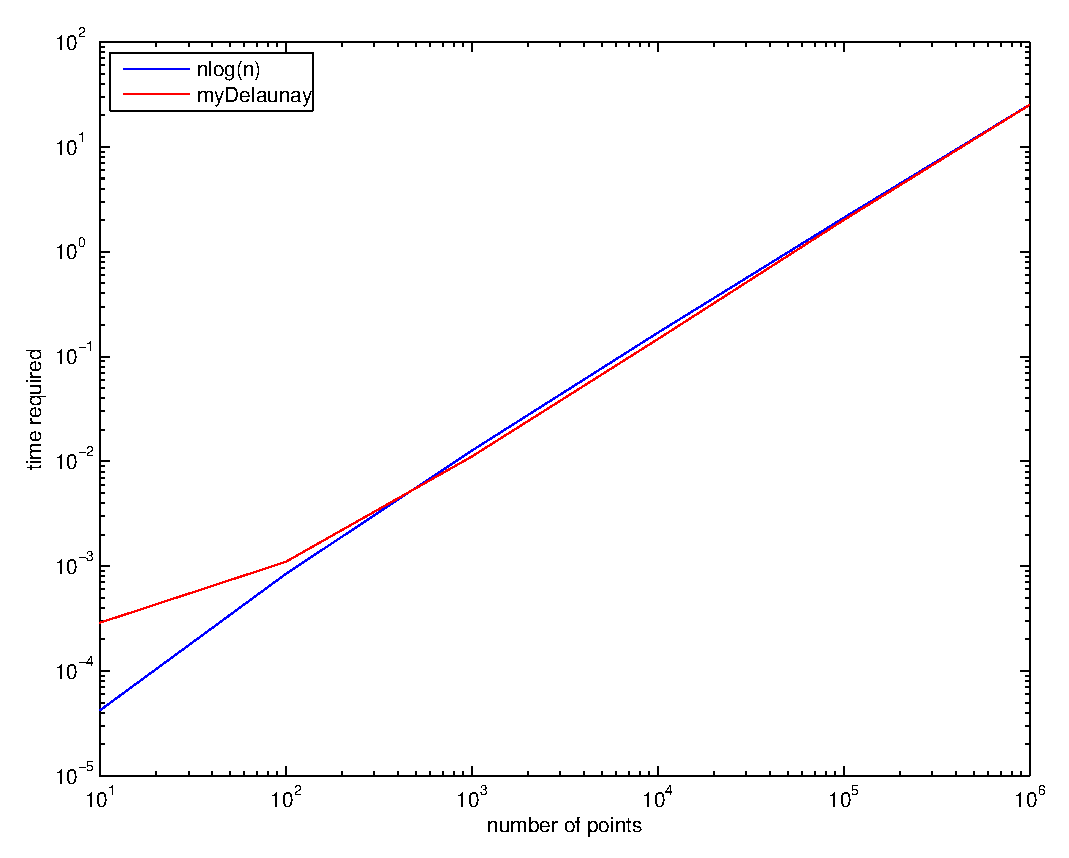
\includegraphics[scale=0.5]{images/timeRandom.eps}
\caption{Computation time (red line) for randomly chosen points from $1e1$ to $1e6$ and theoretical time (blue line) $n\log n$.}
\label{fig:timeRandom}
\end{figure}

As explained earlier we have two types of implementations, a robust one and a less robust one. The table~\ref{tab:proportion} shows the exact times for both implementation and the ratio between them. \cite{shewchuk1996robust} speaks about a $8 \%$ slowdown for orientation 2D in general cases, $30\%$ slowdown for orientation 2D in worst cases and $35\%$ slowdown for in-circle when using their robust implementation. We see that in our case for a sufficient data set we are about $20\%$ slower, quite close from the expected time. 

Moreover, comparing the time for $1e6$ points with the implementation suggested in \cite{triangle}, we have both around $20$ seconds. We don't have the same computer but it shows that we have the same order of magnitude.

The space complexity is theoretically in $\mathcal{O}(n)$, \cite{de2000computational}. Using \texttt{valgrind} we measure the heap memory use at exit. It could seem as we don't think about freeing the memory but the structures we require are used during the whole process and so we can only free at the end. In consequence it's not really strategical and it allows us to easily measure the final space complexity, which is the maximal one. The memory at exit is shown in table \ref{tab:memory}. We see that we have almost the same result as the the theoretical one. Each time we multiply by $10$ we increase the memory used by a factor $10$.

\begin{table}
\centering
\begin{tabular}{c|ccccc}
				& $10^1$ & $10^2$ 	  & $10^3$	 & $10^4$	& $10^5$ \\
				\hline
memory (bytes) & 10,208 & 151,504 & 1,624,304 & 16,513,168 &  165,296,208 \\
\end{tabular}
\caption{Heap memory in use at exit.}
\label{tab:memory}
\end{table}

\begin{table}
\centering
\begin{tabular}{c|cccccc}
	 & $10^1$ & $10^2$ 	 & $10^3$ 	& $10^4$ 	& $10^5$ & $10^6$ \\
	 \hline
not robust &0.0102 & 0.0007 &	0.0062 & 0.1086 &	1.5392 &	20.2006 \\
 robust & 0.01030 &	0.0011 &	0.0096 & 0.1333 &	1.9299 &	25.0801 \\	 
ratio & 0.9903 &  0.6364  &  0.6458   & 0.8147  &  0.7976  &  0.8054\\
\end{tabular}
\caption{Comparison of time between the use of the not robust and robust implementations. }
\label{tab:proportion}
\end{table}

We also implement a script to generate points based on a worst case scenario, \texttt{generatePointLimite.m}. This scenario is a set of points forming a line-sequence of squares. It's considered as a worst case scenario because the points are not spread very uniformly in the space and the points are always exactly on the circle made of the $3$ other points of the square. So the algorithm has a risk of falling into a infinite loop checking a point changing the triangle and then doing it again. In theory the worst case scenario can be in $O(n^2)$ with the Watson algorithm. We see the importance of randomisation in this case. Indeed as shown in figure \ref{fig:timeWorstCaseOrdered}, if we do not randomise the data we are far worse than the theoretical result and if we randomise it, figure \ref{fig:timeWorstCaseRandomised}, we are then close to the theoretical result.  An example of Delaunay triangulation on a sequence of squares is shown in figure \ref{fig:LimitCase}.

\begin{figure}
\centering 
\begin{subfigure}[b]{0.5\textwidth}
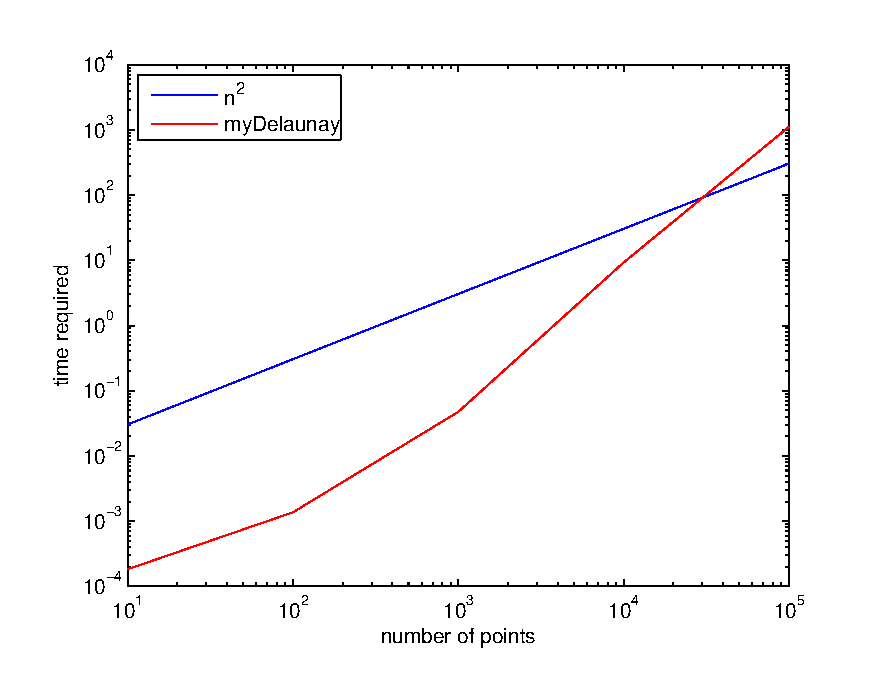
\includegraphics[width=\textwidth]{images/timeWorstCaseOrdered.eps}
\caption{Ordered (only until $10^5$)}
\label{fig:timeWorstCaseOrdered}
\end{subfigure}
~
\begin{subfigure}[b]{0.45\textwidth}
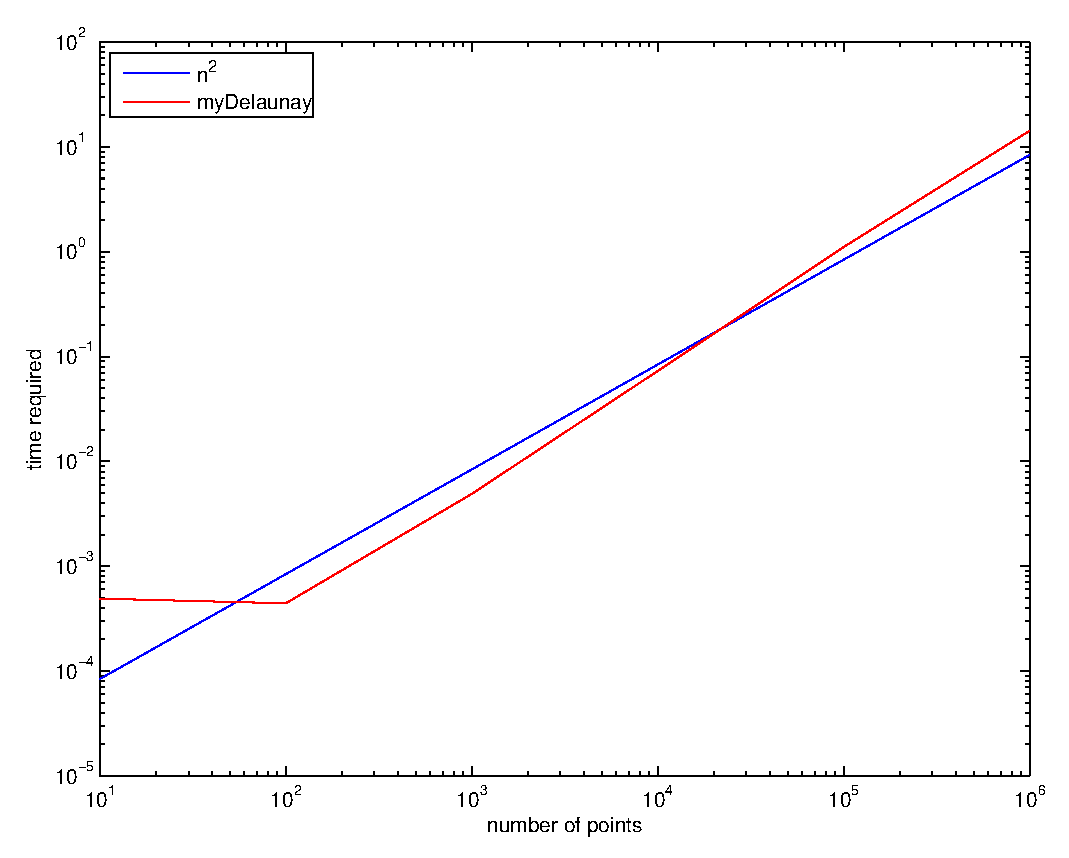
\includegraphics[width=\textwidth]{images/timeWorstCaseRandomised.eps}
\caption{Randomly mixed}
\label{fig:timeWorstCaseRandomised}
\end{subfigure}
\caption{Computation time (red line) for points from $1e1$ to $1e5$ choosen in a worst case scenario and theoretical time (blue line) $n^2$.}
\end{figure}

\begin{figure}
\centering
\begin{subfigure}[b]{0.4\textwidth}
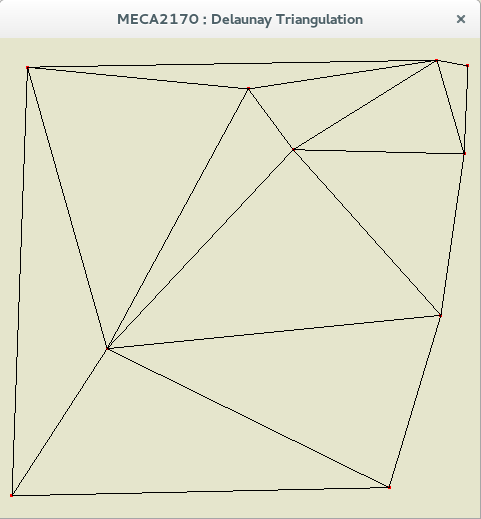
\includegraphics[width=\textwidth]{images/RandomCase.png}
\caption{$10$ random points.}
\label{fig:RandomCase}
\end{subfigure}
~
\begin{subfigure}[b]{0.4\textwidth}
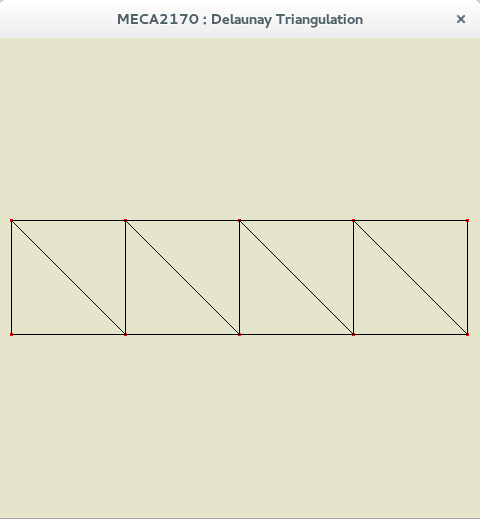
\includegraphics[scale=0.4]{images/worstCase.png}
\caption{$10$ points based on a worst case scenario.}
\label{fig:LimitCase}
\end{subfigure}
\caption{OpenGL representations of some Delaunay Triangulations.}
\end{figure}


A way of improvements would be in the randomised worst case scenario. Indeed in this case we have sometimes some errors due to reasons we didn't get the time to investigate. In short, the algorithm says that the point we want to add is outside of all the triangles. It is obviously not possible as the first triangle contains them all. Note that if we receive a random set of points or an ordered worst case scenario, our algorithm seems like working all the time.